\documentclass{beamer}
%\usepackage{xspace}
\usepackage{amsmath,amssymb}
\usepackage{graphicx}
%\usepackage{svg}
%\usepackage{pgfpages}
%\pgfpagesuselayout{4 on 1}[a4paper,border shrink=5mm,landscape]
%\usepackage{psfrag}
%\usepackage[usenames,dvipsnames]{xcolor}
\usepackage{braket}
\usepackage{tikz}
\usetikzlibrary{graphs}
\usetikzlibrary{datavisualization}
\usetikzlibrary{datavisualization.formats.functions}
\usepackage{pgfplotstable}
\usepgfplotslibrary{patchplots}

\setbeamercovered{transparent}

\usetheme{Pittsburgh}
%\usetheme{default}

\setbeamertemplate{sidebar right}{}
\setbeamertemplate{footline}[frame number]
%\usefonttheme{professionalfonts}

%\usepackage{sansmathaccent}
%\usepackage{bm}

%\usepackage{unicode-math}
%%\setmainfont[SlantedFont={Latin Modern Roman Slanted},SlantedFeatures={Color=000000},
%%  SmallCapsFont={TeX Gyre Termes},SmallCapsFeatures={Letters=SmallCaps}]{XITS}
%\setmathfont[math-style=ISO,sans-style=upright]{XITS Math}
%\setmathfont[range={\mathcal,\mathbfcal}]{Latin Modern Math}

\usepackage{sfmath}

%\mathversion{sans}

\newcommand{\Tr}{\mathsf{Tr}}

\definecolor{redorange}{rgb}{1.0, .25, .25}
\definecolor{citation}{rgb}{.1, 0.8, .35}
\newcommand\emm[1]{\textcolor{redorange}{{#1}}}
\newcommand\numc[1]{\textcolor{citation}{{\bf #1}}}

%\newcommand\bm[1]{{\mbox{\boldmath $#1$}}}
\newcommand\bm[1]{{\mathbf{#1}}}
%\newcommand\bm[1]{{\bf #1}}
%\newcommand\bm[1]{\ensuremath{\boldsymbol{#1}}}
%\newcommand\bm[1]{{\textbf{\it #1}}}

\title{No-signaling polytope and multiplayer XOR games}
\author{Ryuhei Mori}
%\institute{$\vcenter{\hbox{\includegraphics[width=30pt]{ELC_logo}}}$ Postdoctoral Fellow of ELC\\ $\vcenter{\hbox{\includegraphics[width=20pt]{titech_logo}}}$ Tokyo Institute of Technology}
\institute{Tokyo Institute of Technology}
%\date{21, Feb, 2019}



\begin{document}
\begin{frame}[plain]
\maketitle
\end{frame}



\begin{frame}{Bell test: CHSH game (1964, 1969)}
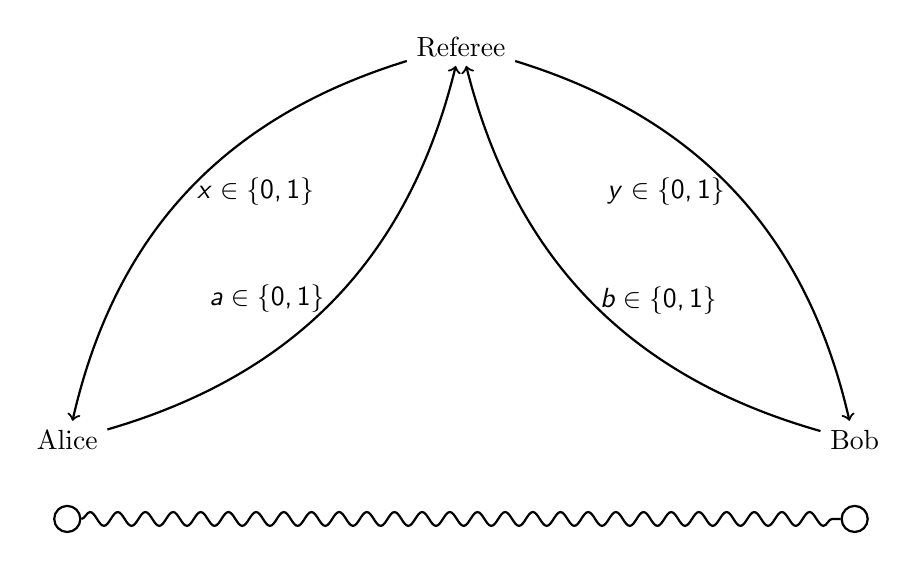
\begin{tikzpicture}
\node at (5,5) (R) {Referee};
\node at (0,0) (A) {Alice};
\node at (10,0) (B) {Bob};
\node at (0,-1)[circle,thick,draw] (As) {};
\node at (10,-1)[circle,thick,draw] (Bs) {};
\draw[->,thick] (R) edge[bend right] node[anchor=west, midway]{$x\in\{0,1\}$} (A);
\draw[->,thick] (R) edge[bend left] node[anchor=east, midway]{$y\in\{0,1\}$} (B);
\draw[->,thick] (A) edge[bend right] node[anchor=east, midway]{$a\in\{0,1\}$} (R);
\draw[->,thick] (B) edge[bend left] node[anchor=west, midway]{$b\in\{0,1\}$} (R);
\draw[thick,decorate,decoration=snake] (As) -- (Bs);
\end{tikzpicture}
%\includegraphics[width=30pt]{Alice_in_Wonderland.png}
\begin{center}
Alice and Bob win iff $\emm{a\oplus b = x\wedge y}$.
\end{center}
\end{frame}


\begin{frame}{Two-party statistics}
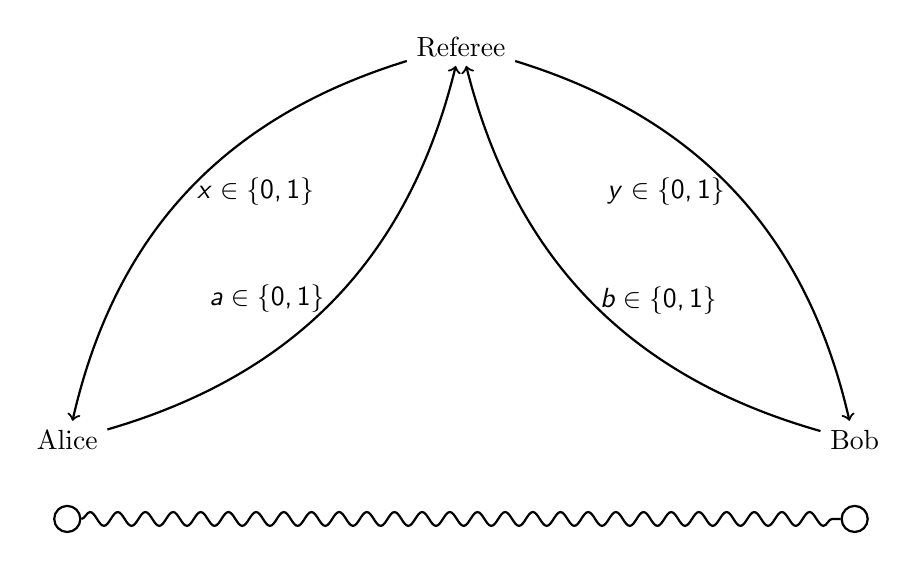
\begin{tikzpicture}
\node at (5,5) (R) {Referee};
\node at (0,0) (A) {Alice};
\node at (10,0) (B) {Bob};
\node at (0,-1)[circle,thick,draw] (As) {};
\node at (10,-1)[circle,thick,draw] (Bs) {};
\draw[->,thick] (R) edge[bend right] node[anchor=west, midway]{$x\in\{0,1\}$} (A);
\draw[->,thick] (R) edge[bend left] node[anchor=east, midway]{$y\in\{0,1\}$} (B);
\draw[->,thick] (A) edge[bend right] node[anchor=east, midway]{$a\in\{0,1\}$} (R);
\draw[->,thick] (B) edge[bend left] node[anchor=west, midway]{$b\in\{0,1\}$} (R);
%\draw[->,thick] (R) edge[bend right] node[anchor=south, midway]{$x$} (A);
%\draw[->,thick] (R) edge[bend left] node[anchor=south, midway]{$y$} (B);
%\draw[->,thick] (A) edge[bend right] node[anchor=north, midway]{$a$} (R);
%\draw[->,thick] (B) edge[bend left] node[anchor=north, midway]{$b$} (R);
\draw[thick,decorate,decoration=snake] (As) -- (Bs);
\end{tikzpicture}
%\includegraphics[width=30pt]{Alice_in_Wonderland.png}
\begin{equation*}
P(a,b\mid x,y), \hspace{2em} \forall a,b\in\{0,1\}, x,y\in\{0,1\}
\end{equation*}
\end{frame}

\begin{frame}{No-signaling condition}
The marginal distribution of $a$ ($b$) \emm{cannot depend on} $y$ ($x$), respectively.
\begin{align*}
\sum_{b\in\{0,1\}} P(a,b\mid x,0) &= \sum_{b\in\{0,1\}} P(a,b\mid x,1),\qquad\forall a,\,x\in\{0,1\}\\
\sum_{a\in\{0,1\}} P(a,b\mid 0,y) &= \sum_{a\in\{0,1\}} P(a,b\mid 1,y),\qquad\forall b,\,y\in\{0,1\}.
\end{align*}
\end{frame}

\begin{frame}{The 8-dimensional linear space and no-signaling polytope}
\small
\begin{align*}
\sum_{a\in\{0,1\},\,b\in\{0,1\}} P(a,b\mid x,y) = 1,\qquad x\in\{0,1\},\, y\in\{0,1\}.
\end{align*}
\begin{align*}
\sum_{b\in\{0,1\}} P(0,b\mid 0,0) &= \sum_{b\in\{0,1\}} P(0,b\mid 0,1)\\
\sum_{b\in\{0,1\}} P(0,b\mid 1,0) &= \sum_{b\in\{0,1\}} P(0,b\mid 1,1)\\
\sum_{a\in\{0,1\}} P(a,0\mid 0,0) &= \sum_{a\in\{0,1\}} P(a,0\mid 1,0)\\
\sum_{a\in\{0,1\}} P(a,0\mid 0,1) &= \sum_{a\in\{0,1\}} P(a,0\mid 1,1).
\end{align*}

\vspace{.5em}
\begin{center}
$16-8=\emm{8}$-dimensional linear space.
\end{center}
\end{frame}

\begin{frame}{No-signaling polytope}
\centering
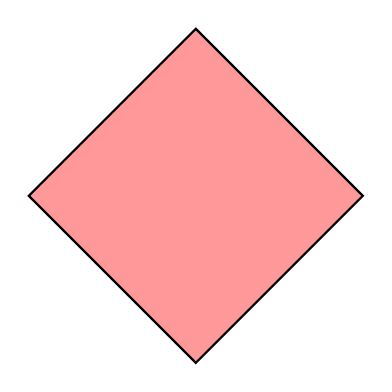
\begin{tikzpicture}
\draw [rotate=45, thick, red!40, fill, draw=black] (-1.5,-1.5) rectangle  (1.5,1.5);
%\draw [thick, green!40, fill] (-1.061,-1.061) rectangle  (1.061,1.061);
\end{tikzpicture}
\end{frame}

\begin{frame}{Local polytope}
\emm{Deterministic} choice
\begin{align*}
a&=A(x),& b&=B(y).
\end{align*}

Local polytope
\begin{align*}
\mathsf{conv}\left(\left\{\left\{P(a,b\mid x,y)=\delta_{(a,b),(A(x),B(y))}\right\}_{a,b,x,y}\mid A, B\in\{0,1\}^{\{0,1\}}\right\}\right).
\end{align*}

\end{frame}

\begin{frame}{No-signaling polytope and local polytope}
\centering
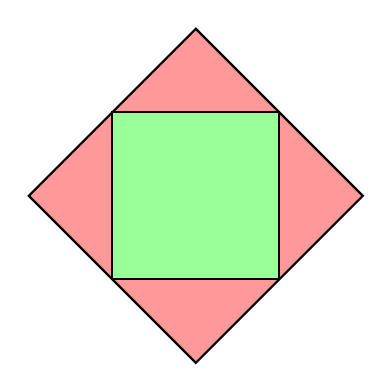
\begin{tikzpicture}
%\draw [fill, black!50] (0,0) circle [radius=1.5cm];
%\draw (-1.061,-1.061) rectangle (1.061,1.061);
\draw [rotate=45, thick, red!40, fill, draw=black] (-1.5,-1.5) rectangle  (1.5,1.5);
\draw [thick, green!40, fill, draw=black] (-1.061,-1.061) rectangle  (1.061,1.061);
%\draw [dashed,thick] (-1.061*2, 1.5) to (1.061*2, 1.5) node[right] {CHSH probability $ \approx 0.854$};
%\draw [dashed,thick] (-1.061*2, 1.061*2) to (1.061*2, 1.061*2) node[right] {CHSH probability $ = 1$};
%\draw (5.5,-0.5) node [align=left, text width = 5.9cm ] (T) {ESC$BNL;RNO3X$K$h$C$F@8@.$5$l$kAj4X$N=89g!#ESC(B\\ \textbf{ESC$B$3$N=89g$r!VA`:nE*0UL#$N$"$k>r7o$G!WFCD'IU$1$?$$ESC(B}};
%\draw [->,thick] (2.5,-0.2) node [right, align=left, text width = 5.9cm ] {ESC$BNL;RNO3X$K$h$C$F@8@.$5$l$kAj4X$N=89g!#ESC(B\\ \textbf{ESC$B$3$N=89g$r!VA`:nE*0UL#$N$"$k>r7o$G!WFCD'IU$1$?$$ESC(B}} to (1.5,0.2);
%\draw [-{Stealth[length=2.5mm]},thick] (T.west) to (1.5,-0.2);
%\draw [-{Stealth[length=2.5mm]},thick] (-2.5,0.5) node [left, align=left, text width = 5.2cm ] {No-signaling ESC$B>r7o$N$_$rK~$?$9Aj4X$N=89gESC(B} to (-1.85,0.3);
\end{tikzpicture}
\end{frame}

\begin{frame}{CHSH inequality: Facets of the local polytope}
\begin{align*}
\emm{\sum_{a\oplus b=x\wedge y} P(a,b\mid x,y) }\ &\emm{\le 3},&
\sum_{a\oplus b\ne x\wedge y} P(a,b\mid x,y) &\le 3\\
\sum_{a\oplus b=\overline{x}\wedge y} P(a,b\mid x,y) &\le 3,&
\sum_{a\oplus b\ne \overline{x}\wedge y} P(a,b\mid x,y) &\le 3\\
\sum_{a\oplus b=x\wedge \overline{y}} P(a,b\mid x,y) &\le 3,&
\sum_{a\oplus b\ne x\wedge \overline{y}} P(a,b\mid x,y) &\le 3\\
\sum_{a\oplus b=\overline{x}\wedge \overline{y}} P(a,b\mid x,y) &\le 3,&
\sum_{a\oplus b\ne \overline{x}\wedge \overline{y}} P(a,b\mid x,y) &\le 3
\end{align*}
 CHSH inequality [{Clauser, Horne, Shimony, Holt} 1969].

CHSH inequality is the only non-trivial facets [Froissard 1981], [Fine 1982].
\end{frame}



\begin{frame}{No-signaling condition admits CHSH probability 1}
%\begin{align*}
%P(a = 0, b = 0\mid x=0, y = 0) &=
%P(a = 1, b = 1\mid x=0, y = 0) = 1/2\\
%P(a = 0, b = 0\mid x=0, y = 1) &=
%P(a = 1, b = 1\mid x=0, y = 1) = 1/2\\
%P(a = 0, b = 0\mid x=1, y = 0) &=
%P(a = 1, b = 1\mid x=1, y = 0) = 1/2\\
%P(a = 0, b = 1\mid x=1, y = 1) &=
%P(a = 1, b = 0\mid x=1, y = 1) = 1/2
%\end{align*}

\begin{align*}
P(0, 0\mid 0, 0) &=
P(1, 1\mid 0, 0) = 1/2\\
P(0, 0\mid 0, 1) &=
P(1, 1\mid 0, 1) = 1/2\\
P(0, 0\mid 1, 0) &=
P(1, 1\mid 1, 0) = 1/2\\
P(0, 1\mid 1, 1) &=
P(1, 0\mid 1, 1) = 1/2
\end{align*}

\vspace{1em}
\begin{center}
PR box

[Popescu and  Rohrlich 1994]
\end{center}
\end{frame}

\begin{frame}{No-signaling polytope, local polytope and quantum correlation}
\centering
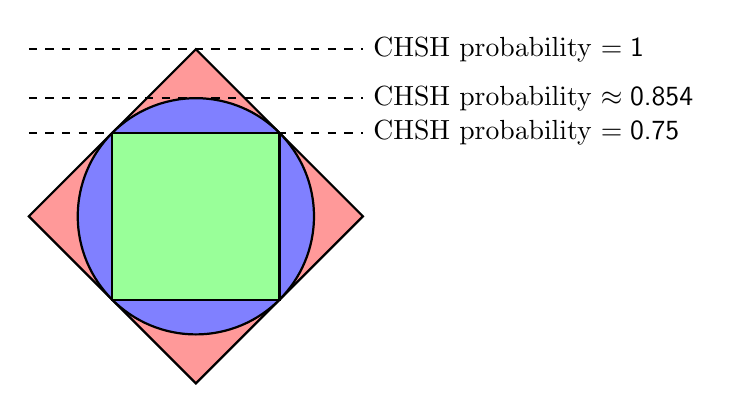
\begin{tikzpicture}
%\draw (-1.061,-1.061) rectangle (1.061,1.061);
\draw [rotate=45, thick, red!40, fill, draw=black] (-1.5,-1.5) rectangle  (1.5,1.5);
\draw [blue!50, fill, thick, draw=black] (0,0) circle [radius=1.5cm];
\draw [thick, green!40, fill, draw=black] (-1.061,-1.061) rectangle  (1.061,1.061);
\draw [dashed,thick] (-1.061*2, 1.5) to (1.061*2, 1.5) node[right] {CHSH probability $ \approx 0.854$};
\draw [dashed,thick] (-1.061*2, 1.061*2) to (1.061*2, 1.061*2) node[right] {CHSH probability $ = 1$};
\draw [dashed,thick] (-1.061*2, 1.061) to (1.061*2, 1.061) node[right] {CHSH probability $ = 0.75$};
%\draw (5.5,-0.5) node [align=left, text width = 5.9cm ] (T) {ESC$BNL;RNO3X$K$h$C$F@8@.$5$l$kAj4X$N=89g!#ESC(B\\ \textbf{ESC$B$3$N=89g$r!VA`:nE*0UL#$N$"$k>r7o$G!WFCD'IU$1$?$$ESC(B}};
%\draw [->,thick] (2.5,-0.2) node [right, align=left, text width = 5.9cm ] {ESC$BNL;RNO3X$K$h$C$F@8@.$5$l$kAj4X$N=89g!#ESC(B\\ \textbf{ESC$B$3$N=89g$r!VA`:nE*0UL#$N$"$k>r7o$G!WFCD'IU$1$?$$ESC(B}} to (1.5,0.2);
%\draw [-{Stealth[length=2.5mm]},thick] (T.west) to (1.5,-0.2);
%\draw [-{Stealth[length=2.5mm]},thick] (-2.5,0.5) node [left, align=left, text width = 5.2cm ] {No-signaling ESC$B>r7o$N$_$rK~$?$9Aj4X$N=89gESC(B} to (-1.85,0.3);
\end{tikzpicture}

\vspace{1em}
\centering
Question:

\vspace{.5em}
\bfseries
Why does quantum physics prohibits CHSH probability greater than $\mathbf{(2+\sqrt{2})/4\approx0.854}$ ?
\end{frame}

%\begin{frame}{Principles}
%\end{frame}

\begin{frame}{Multiplayer XOR game}
\begin{itemize}
\setlength{\itemsep}{2em}
\item $n$ players.
\item $j$-th player are given $x_j\in\mathcal{X}$ according to a probability distribution $p(x_1,\dotsc,x_n)$.
\item $j$-th player outputs $a^{(j)}$.
\item Players win iff $\emm{\bigoplus_{j=1}^n}\, a^{(j)} = f(x_1,\dotsc,x_n)$.
\end{itemize}

\vspace{1em}
Example: Mermin--GHZ game
\begin{itemize}
\setlength{\itemsep}{1em}
\item 3 players.
\item $\mathcal{X}=\{0,1\}$. $p(x_1,x_2,x_3) = 1/4$ for $x_1\oplus x_2\oplus x_3=0$.
\item $f(x_1,x_2,x_3) = x_1\vee x_2\vee x_3$.
\end{itemize}
\end{frame}

\begin{frame}{The winning condition for Mermin--GHZ game}
\begin{align*}
a_0\oplus b_0 \oplus c_0 &= 0\\
a_1\oplus b_0 \oplus c_1 &= 1\\
a_0\oplus b_1 \oplus c_1 &= 1\\
a_1\oplus b_1 \oplus c_0 &= 1
\end{align*}
The sum is $0=1$ which means that there is no solution in the above system of linear equations.
The largest classical winning probability is 3/4.

\vspace{2em}
\centering
Quantum theory allows the winning probability \emm{1}\\
(Mermin--GHZ paradox).
\end{frame}

\begin{frame}{Observables for XOR game}
For a single qubit projective measurement $\{\ket{\psi_0}\bra{\psi_0}, \ket{\psi_1}\bra{\psi_1}\}$,
we can define an observable $\emm{A := \ket{\psi_0}\bra{\psi_0} - \ket{\psi_1}\bra{\psi_1}}$.
Then, $\Tr(\rho \ket{\psi_x}\bra{\psi_x}) = (1+(-1)^x\Tr(\rho \emm{A}))/2$. Especially,
\begin{align*}
\Tr(\rho \emm{A}) = 1 &\iff \Tr(\rho \ket{\psi_0}\bra{\psi_0}) = 1\\
\Tr(\rho \emm{A}) = -1 &\iff \Tr(\rho \ket{\psi_1}\bra{\psi_1}) = 1.
\end{align*}

For multiple qubits,
\begin{align*}
\Tr\left(\rho \bigotimes_{j=1}^n\emm{A_j}\right) = 1 &\iff \sum_{x:\,|x|\text{ is even}}\Tr\left(\rho \bigotimes_{j=1}^n\ket{\psi_{x_j}}\bra{\psi_{x_j}}\right) = 1\\
\Tr\left(\rho \bigotimes_{j=1}^n\emm{A_j}\right) = -1 &\iff \sum_{x:\,|x|\text{ is odd}}\Tr\left(\rho \bigotimes_{j=1}^n\ket{\psi_{x_j}}\bra{\psi_{x_j}}\right) = 1
\end{align*}
since the eigenvectors of $\bigotimes_{j=1}^n \emm{A_j}$ is $\ket{\psi^{(1)}_{x_1}}\ket{\psi^{(2)}_{x_2}}\dotsm \ket{\psi^{(n)}_{x_n}}$ with eigenvalue $(-1)^{x_1+\dotsb+x_n}$ for $x_1\dotsm x_n\in\{0,1\}^n$.
\end{frame}

\begin{frame}{The quantum strategy for Mermin--GHZ game}
\begin{itemize}
\setlength{\itemsep}{1em}
\item The GHZ state is shared.
\begin{equation*}
\ket{\mathsf{GHZ}}:=\frac1{\sqrt{2}}(\ket{000}+\ket{111}).
\end{equation*}
%\item Alice, Bob and Charlie measure their state by $\{\ket{+}, \ket{-}\}$ if the input is 0, and by $\{\ket{0}+i\ket{1}, \ket{0}-i\ket{1}\}$ if the input is 1.
\item Alice, Bob and Charlie measure their state by $\emm{X}$ if the input is 0, and by $\emm{Y}$ if the input is 1.
\item If $x_1=x_2=x_3=0$, $\bra{\mathsf{GHZ}} \emm{X}^{\otimes 3}\ket{\mathsf{GHZ}}=1$.
\item If $x_1=x_2=1,\,x_3=0$, $\bra{\mathsf{GHZ}} \emm{Y}^{\otimes 2}\otimes \emm{X}\ket{\mathsf{GHZ}}=-1$.
%$a=(a^{(1)})$ is measured with probability $|\bra{a^{(1)}a^{(2)}a^{(3)}}H^{\otimes 3}\ket{\mathsf{GHZ}}|^2 = \frac12 (\frac1{2\sqrt{2}}(1 + (-1)^{a^{(1)}+a^{(2)}+a^{(3)}}))^2$.
\item This means that the winning probability of the Mermin--GHZ game is 1.
\end{itemize}
\end{frame}

\begin{frame}{The optimal strategy for multiplayer XOR game with binary inptus}
In the following, we consider general multiplayer XOR games with binary inptus ($\mathcal{X}=\{0,1\}$).

\vspace{2em}
\begin{itemize}
\setlength{\itemsep}{1em}
\item The generalized GHZ state is shared.
\begin{equation*}
\ket{\mathsf{GHZ}_n}:=\frac1{\sqrt{2}}(\ket{0\dotsm 0}+\ket{1\dotsm 1}).
\end{equation*}
\item $j$-th player measures his or her qubit by $\emm{\cos\theta_0^{(j)} X + \sin\theta_0^{(j)} Y}$ if the input is 0, and by $\emm{\cos\theta_1^{(j)} X + \sin\theta_1^{(j)} Y}$ if the input is 1.
\end{itemize}
\end{frame}



\begin{frame}{The winning probability {\small [Werner \& Wolf 2001]}}
\small
\begin{align*}
&\Tr\left(\ket{\mathsf{GHZ}_n}\bra{\mathsf{GHZ}_n}\bigotimes_{j=1}^n(\cos \theta_{x_j}^{(j)} X + \sin \theta_{x_j}^{(j)} Y)\right)\\
&= \frac12\sum_{z\in\{0,1\}}\prod_{j=1}^n \left(\cos \theta_{x_j}^{(j)} \bra{z}X\ket{\bar{z}} + \sin \theta_{x_j}^{(j)}\bra{z}Y\ket{\bar{z}}\right)\\
&= \frac12\sum_{z\in\{0,1\}}\prod_{j=1}^n \left(\cos \theta_{x_j}^{(j)} + \sin \theta_{x_j}^{(j)} (-1)^{z}i\right)\\
&= \frac12\sum_{z\in\{0,1\}}\prod_{j=1}^n \exp\left\{(-1)^z \theta_{x_j}^{(j)}\right\}\\
&= \frac12\left(\exp\left\{i\sum_{j=1}^n \theta_{x_j}^{(j)}\right\} + \exp\left\{-i\sum_{j=1}^n \theta_{x_j}^{(j)}\right\}\right)\\
&= \cos\left\{\sum_{j=1}^n \theta_{x_j}^{(j)}\right\}
\end{align*}
\end{frame}

\begin{frame}{Spectral norm}
For $A\in L(\mathbb{C}^n, \mathbb{C}^m)$,
\begin{align*}
\|A\| := \max_{\ket{\psi}\in\mathbb{C}^n\colon \braket{\psi|\psi}=1}\sqrt{\bra{\psi}A^\dagger A\ket{\psi}}
\end{align*}
$\|A\|$ is the largest singular value of $A$.

\vspace{2em}
For any unitary matrices $\emm{U}\in L(\mathbb{C}^m)$ and $\emm{V}\in L(\mathbb{C}^n)$,
\begin{align*}
\|\emm{U}A\emm{V}\| = \|A\|.
\end{align*}
\end{frame}

\begin{frame}{\large The upper bound of the winning probability {\scriptsize [Werner \& Wolf 2001]}}
\scriptsize
Let $\beta(x_1,\dotsc,x_n):=p(x_1,\dotsc,x_n)(-1)^{f(x_1,\dotsc,x_n)}$ and $U_j = A_j^{(0)}A_j^{(1)}$.
\begin{align*}
&\sum_{x_1,\dotsc,x_n}\beta(x_1,\dotsc,x_n)\Tr\left(\rho\bigotimes_{j=1}^n A_j^{(x_j)}\right)
=\sum_{x_1,\dotsc,x_n}\beta(x_1,\dotsc,x_n)\bra{\psi}\bigotimes_{j=1}^n A_j^{(x_j)}\ket{\psi}\\
&=\bra{\psi}\sum_{x_1,\dotsc,x_n}\beta(x_1,\dotsc,x_n)\bigotimes_{j=1}^n A_j^{(x_j)}\ket{\psi}
\le\left\|\sum_{x_1,\dotsc,x_n}\beta(x_1,\dotsc,x_n)\bigotimes_{j=1}^n A_j^{(x_j)}\right\|\\
&=\left\|\bigotimes_{j=1}^nA_j^{(0)}\sum_{x_1,\dotsc,x_n}\beta(x_1,\dotsc,x_n)\bigotimes_{j=1}^n U_j^{x_j}\right\|
%&=\left\|\sum_{x_1,\dotsc,x_n}\beta(x_1,\dotsc,x_n)\bigotimes_{j=1}^nA_j^{(0)}\bigotimes_{j=1}^n U_j^{x_j}\right\|\\
=\left\|\sum_{x_1,\dotsc,x_n}\beta(x_1,\dotsc,x_n)\bigotimes_{j=1}^n U_j^{x_j}\right\|\\
&\le\max_{\theta_1,\dotsc,\theta_n}\left|\sum_{x_1,\dotsc,x_n}\beta(x_1,\dotsc,x_n)\exp\left\{i\sum_{j=1}^n x_j\theta_j\right\}\right|\\
&=\max_{\theta_0,\dotsc,\theta_n}\sum_{x_1,\dotsc,x_n}\beta(x_1,\dotsc,x_n)\cos\left\{\theta_0 + \sum_{j=1}^n x_j\theta_j\right\}.
%&=\left\|\sum_{x_1,\dotsc,x_n}p(x_1,\dotsc,x_n)\bigotimes_{j=1}^n \begin{bmatrix}1&0&\dotsm\\0&\mathsf{e}&\dotsm\end{bmatrix}\right\|\\
\end{align*}
The strategy with $\theta_{x}^{(j)}:= \theta_0/n + x\theta_j$ achieves this bound.
\end{frame}

\begin{frame}{Existence of winning strategies of multiplayer XOR game}
A classical winning strategy exists iff
there exists $(a_x^{(j)}\in\emm{\mathbb{F}_2})_{j=1,\dotsc,n,\,x\in\mathcal{X}}$
such that
\begin{align*}
\sum_{j=1}^n a^{(j)}_{x_j} = f(x_1,\dotsc,x_n) \mod 2
\end{align*}
for all $x\in\mathsf{supp}(p)$.

\vspace{2em}
When \emm{$\mathcal{X}=\{0,1\}$},\\
a quantum winning strategy exists iff
there exists $(\theta_x^{(j)}\in\emm{\mathbb{Q}})_{j=1,\dotsc,n,\,x\in\mathcal{X}}$
such that
\begin{align*}
\sum_{j=1}^n \theta^{(j)}_{x_j} = f(x_1,\dotsc,x_n) \mod 2
\end{align*}
for all $x\in\mathsf{supp}(p)$.
\end{frame}

\begin{frame}{Assignments}
\begin{enumerate}
\setlength{\itemsep}{2em}
\item Show that the PR-box satisfies the no-signaling condition.
\item Show an optimal strategy for the generalized Mermin--GHZ game, defined by
\small
\begin{align*}
p(x_1,\dotsc,x_n) &:= \frac{\mathbb{I}\left\{\sum_{j=1}^n x_j\text{ is divisible by } 2^\ell\right\}}{\left|\left\{z\in\{0,1\}^n\mid \sum_{j=1}^n z_j \equiv 0 \mod 2^\ell\right\}\right|},\\
f(x_1,\dotsc,x_n) &:= \frac{\sum_{j=1}^n x_j}{2^\ell}\mod 2.
\end{align*}
\end{enumerate}
\end{frame}

\end{document}
